\chapter{Wireframe}
\label{cha:Wireframe}

Um \textit{wireframe} é um protótipo da interface do sistema, que serve para ilustrar o funcionamento e interação do usuário com o sistema. A seguir estão três telas do sistema: a página inicial, a página de criação de grade horária, e a página de avaliação de disciplinas e professores. Essas são as principais páginas do sistema.

O design da página inicial (\textit{Landing Page}), apresentado na figura \ref{fig:wireframe-pagina-inicial}, busca ser simples, com uma rápida descrição do sistema e das suas funcionalidades, e com duas opções grandes para enviar o usuário para a página de criação de grade ou de avaliação.

\begin{figure}[ht]
    \begin{center}
    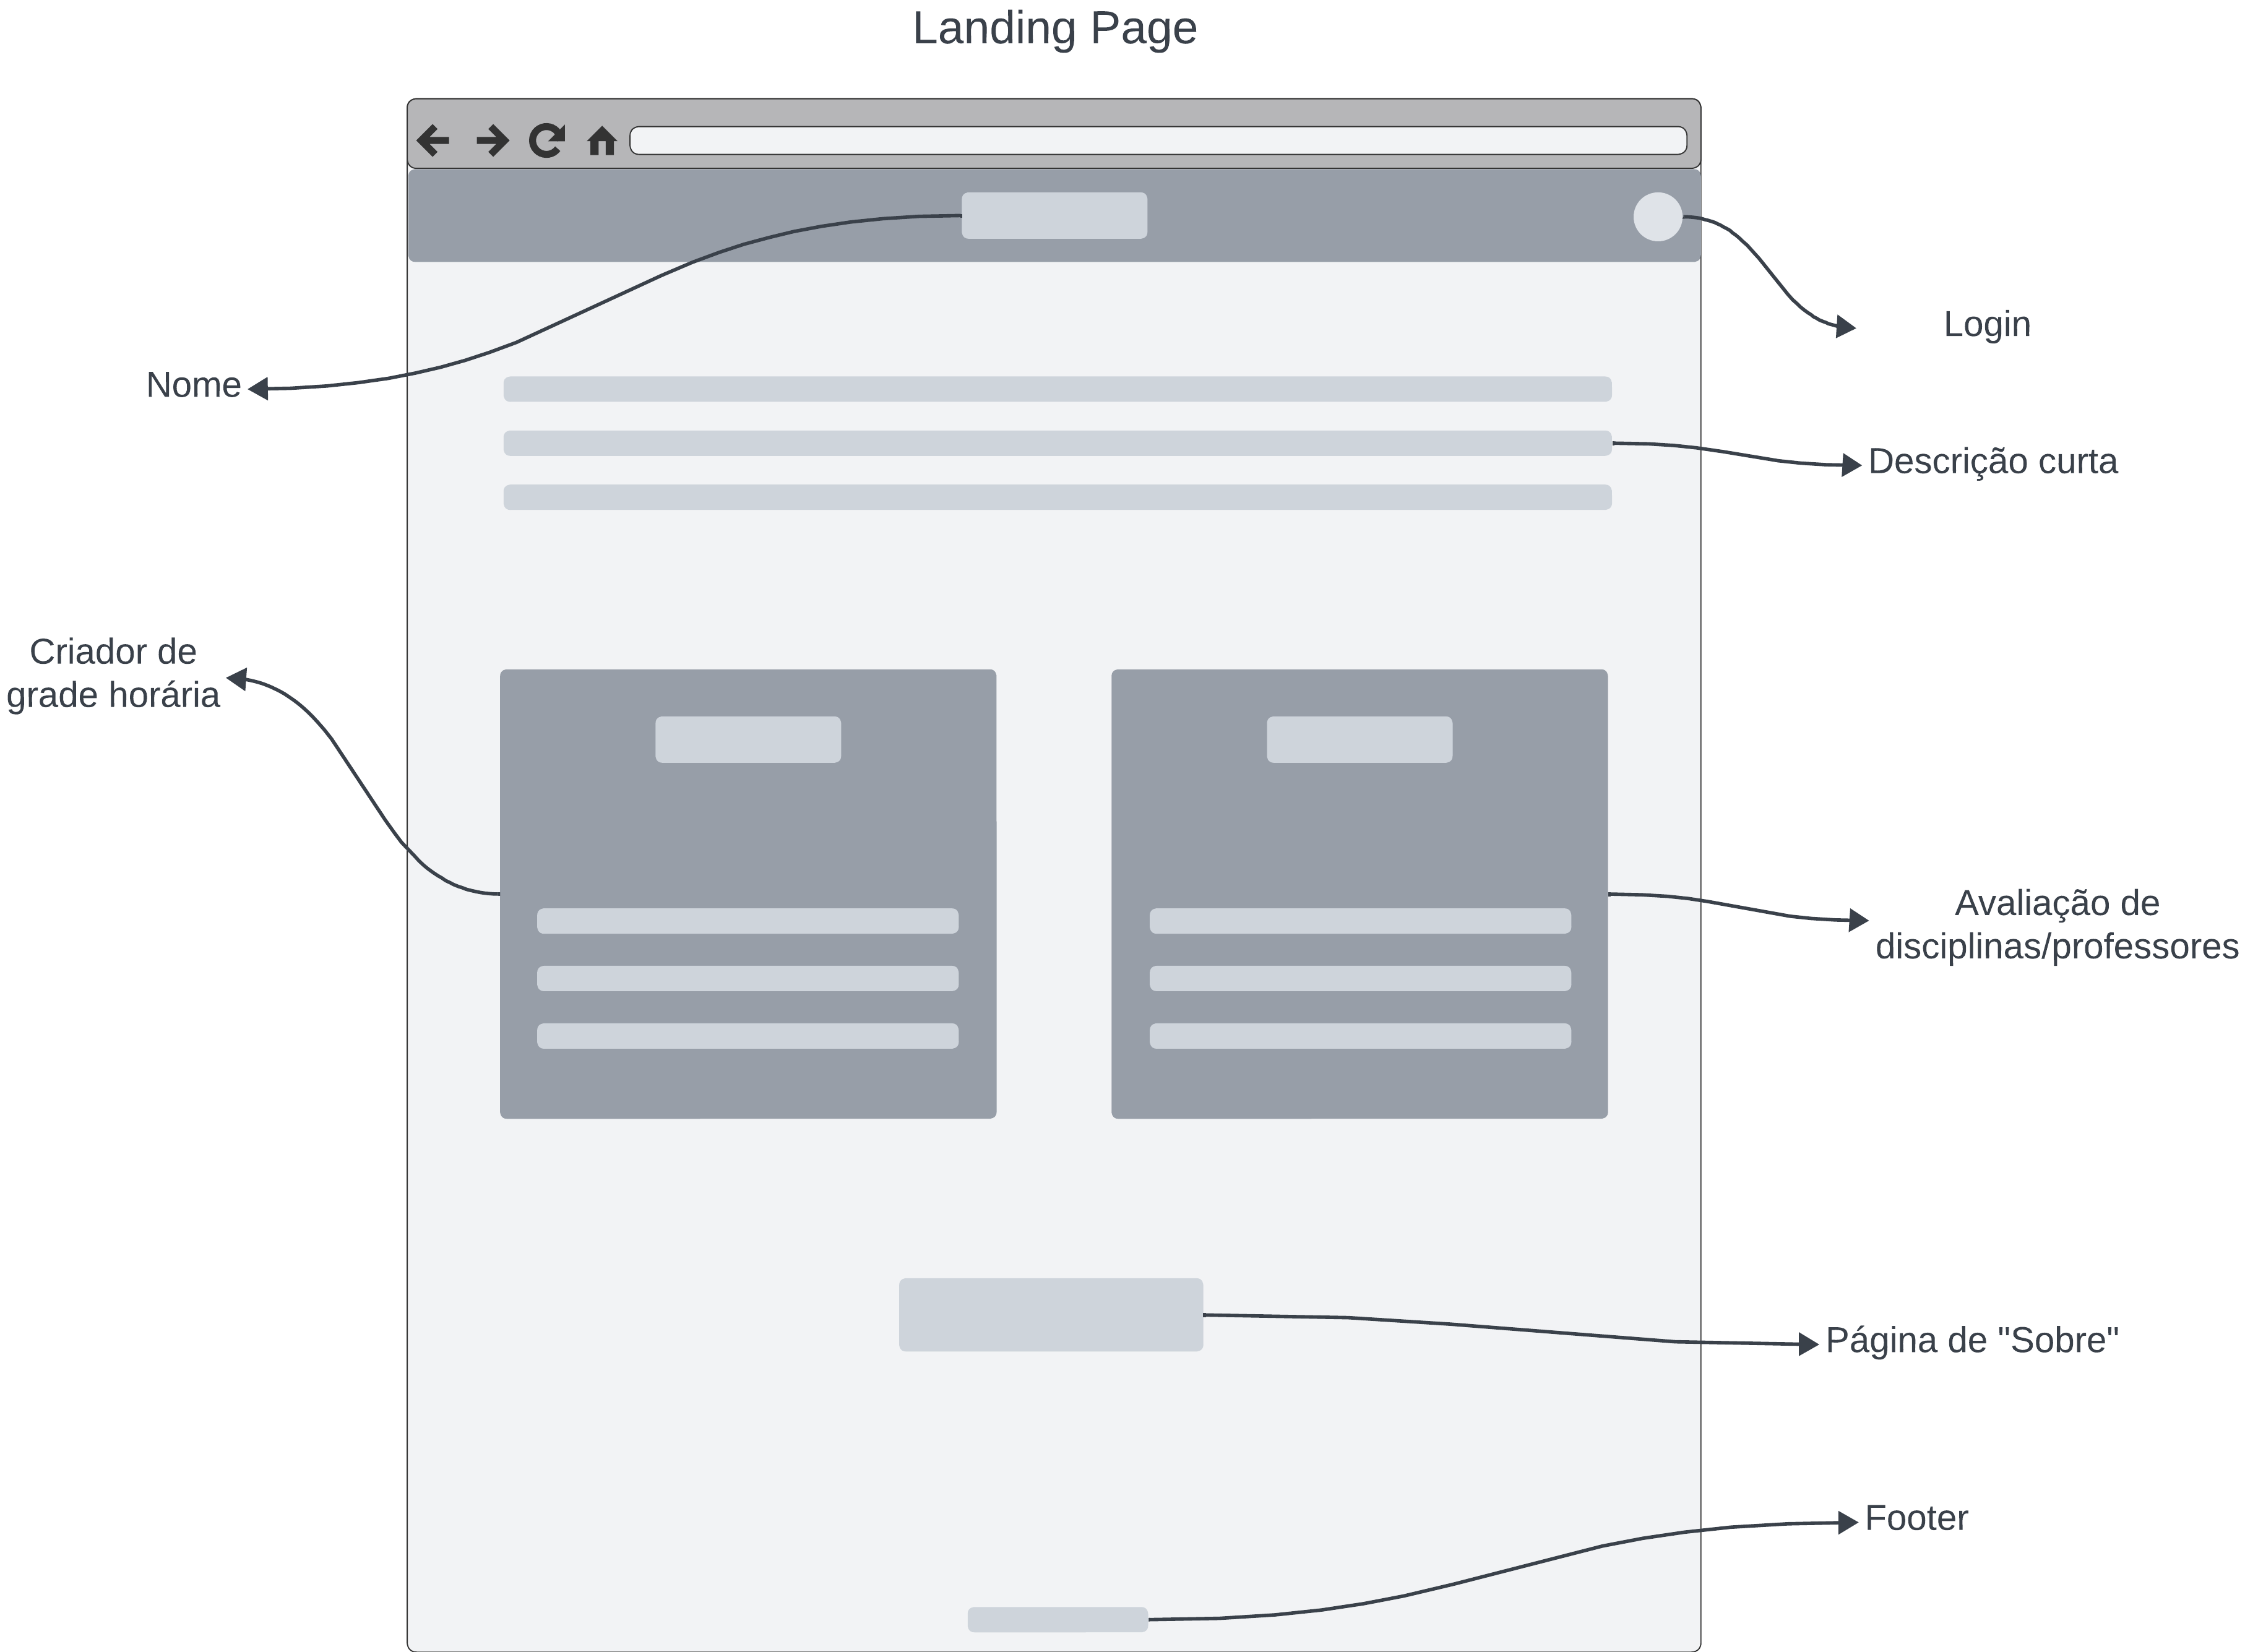
\includegraphics[width=390pt]{figuras/pagina-inicial.png}
    \caption{Wireframe da página inicial (\textit{Landing Page})}
    \label{fig:wireframe-pagina-inicial}
    \end{center}
\end{figure}

A página de criação de grade horária, apresentado na figura \ref{fig:wireframe-pagina-criacao}, pretende ser semelhante à interface de matrícula real da faculdade, como na figura \ref{fig:simulador}, com a adição de mais informações que auxiliem o usuário a fazer suas escolhas, além da barra de disciplinas recomendadas.

\begin{figure}[ht]
    \begin{center}
    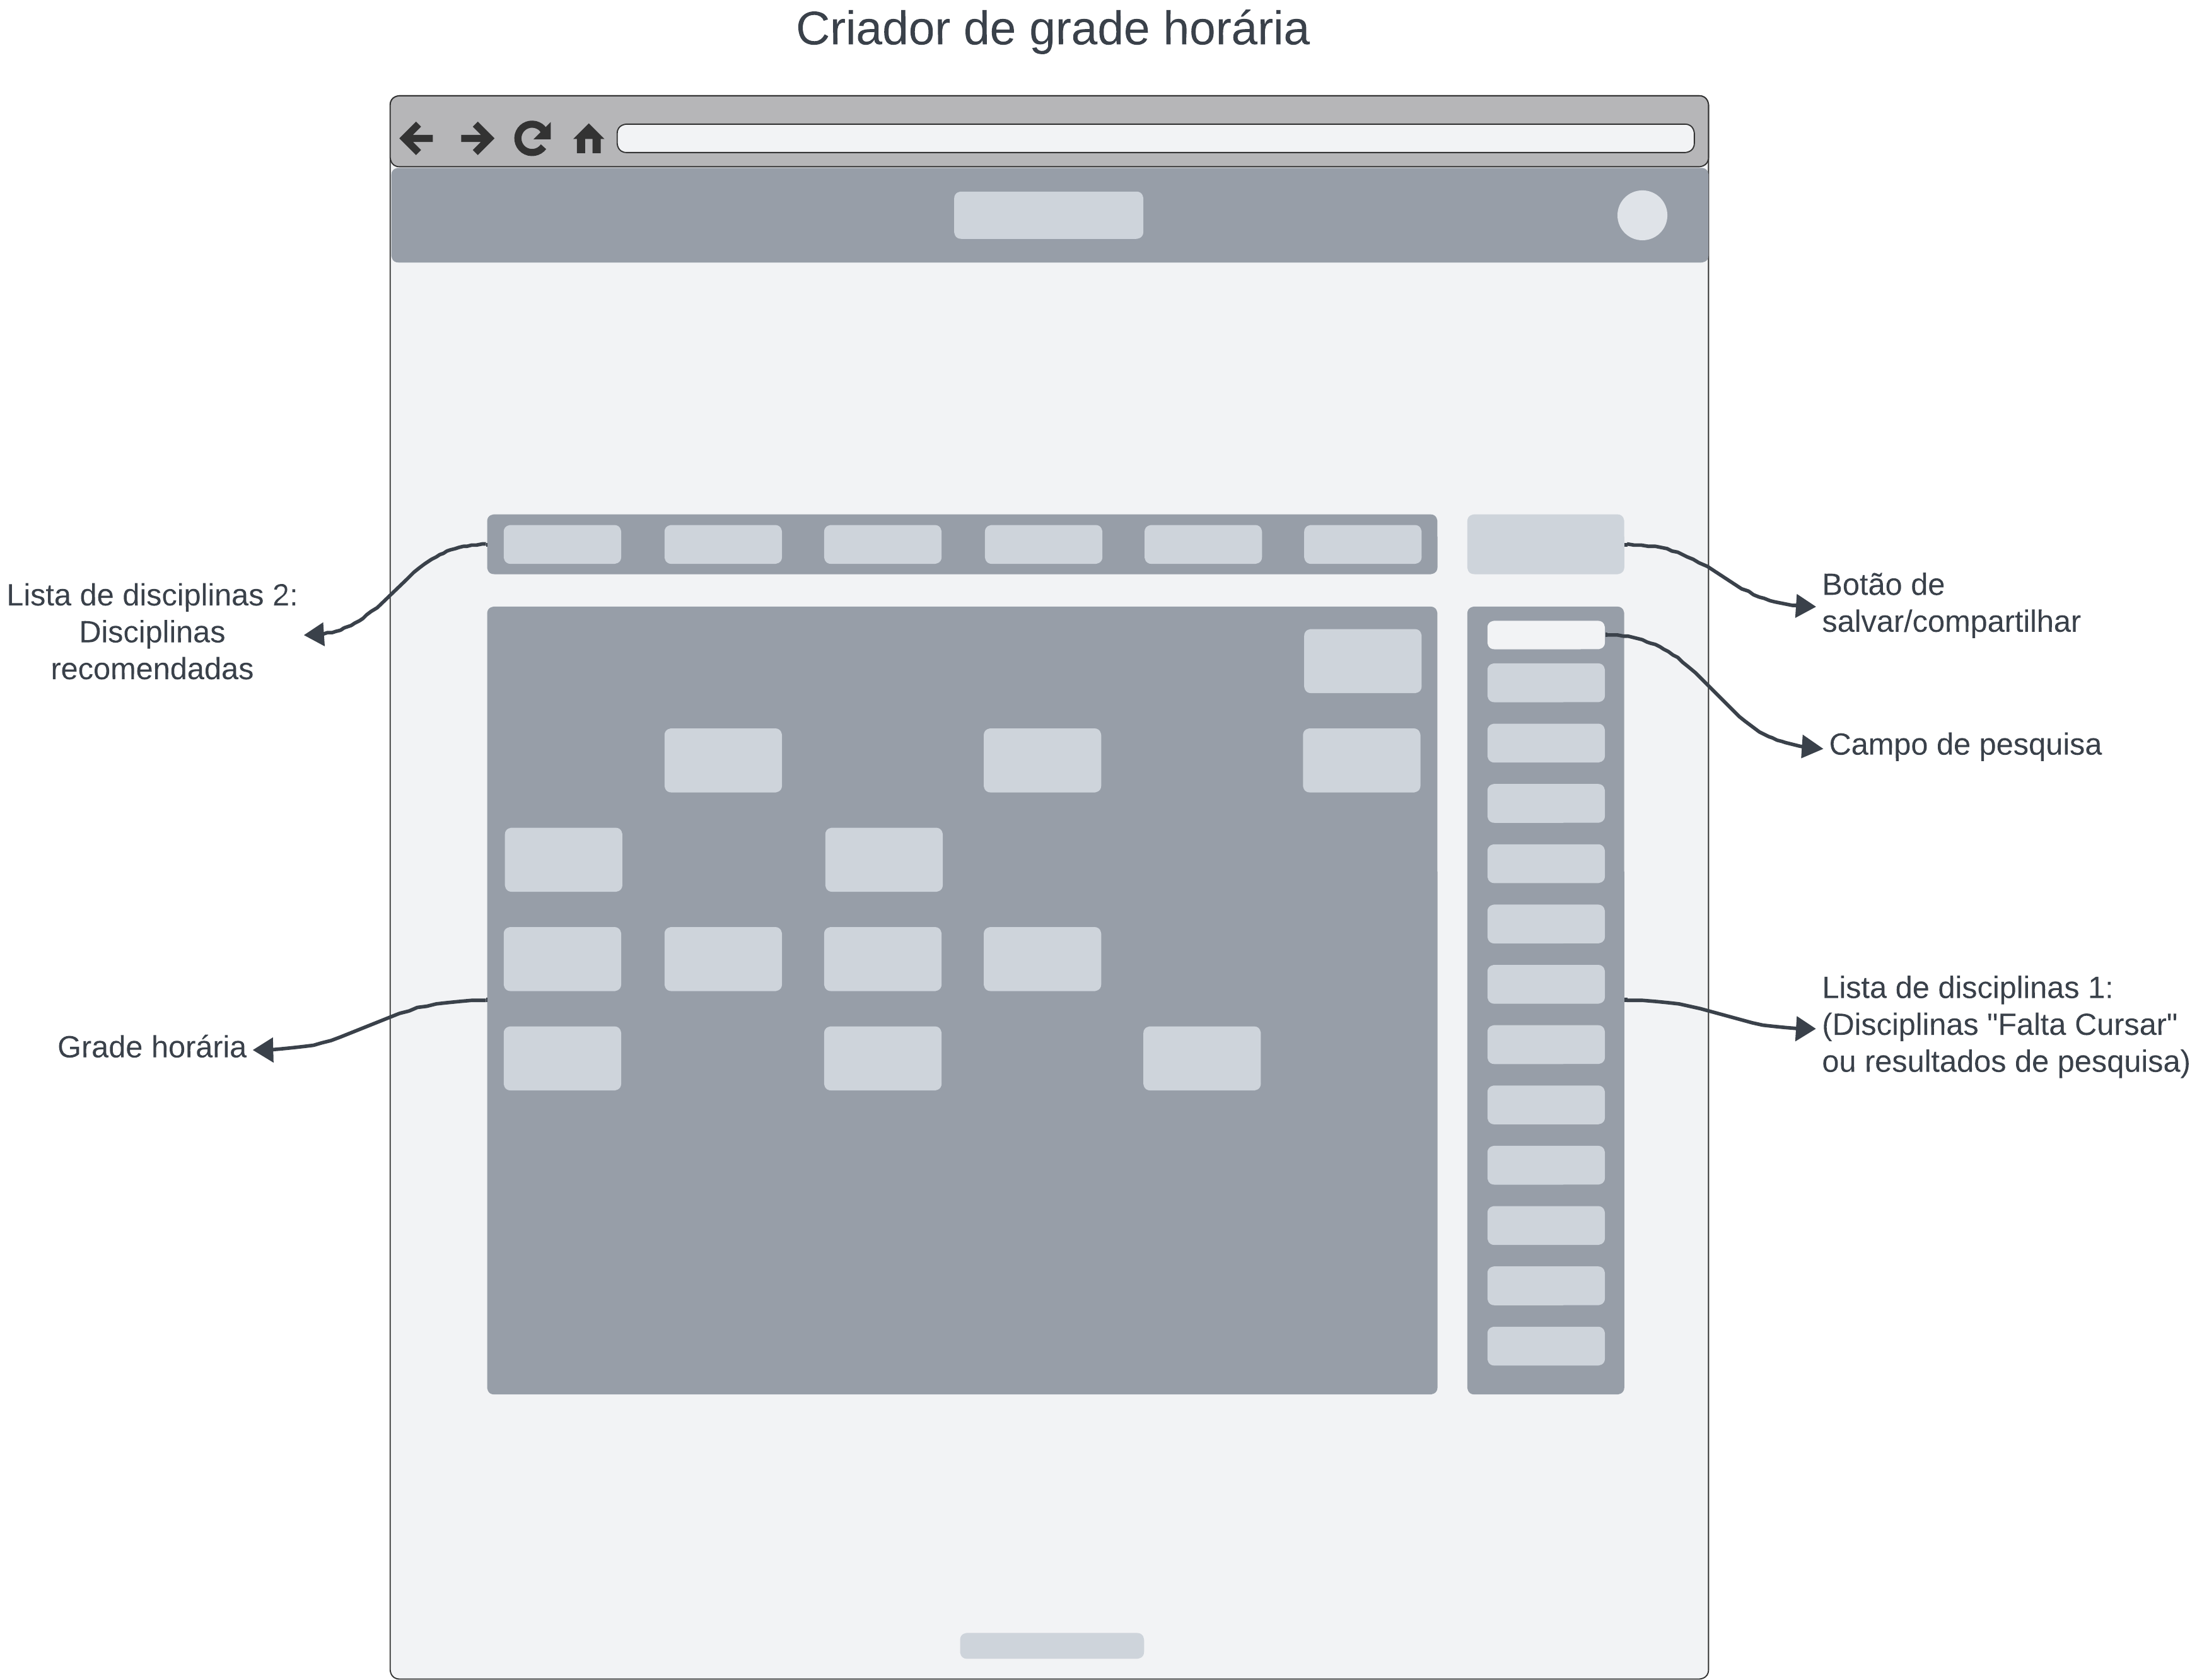
\includegraphics[width=390pt]{figuras/pagina-criacao.png}
    \caption{Wireframe da página de criação de grade horária}
    \label{fig:wireframe-pagina-criacao}
    \end{center}
\end{figure}

Por fim, a página de avaliação de disciplinas e professores, apresentado na figura \ref{fig:wireframe-pagina-avaliacao}, procura ser uma interface simples, com uma lista das disciplinas cursadas ou professores, e com a opção de avaliar no formato de estrelas, sendo a pior avaliação uma estrela, e cinco estrelas a melhor.

\begin{figure}[ht]
    \begin{center}
    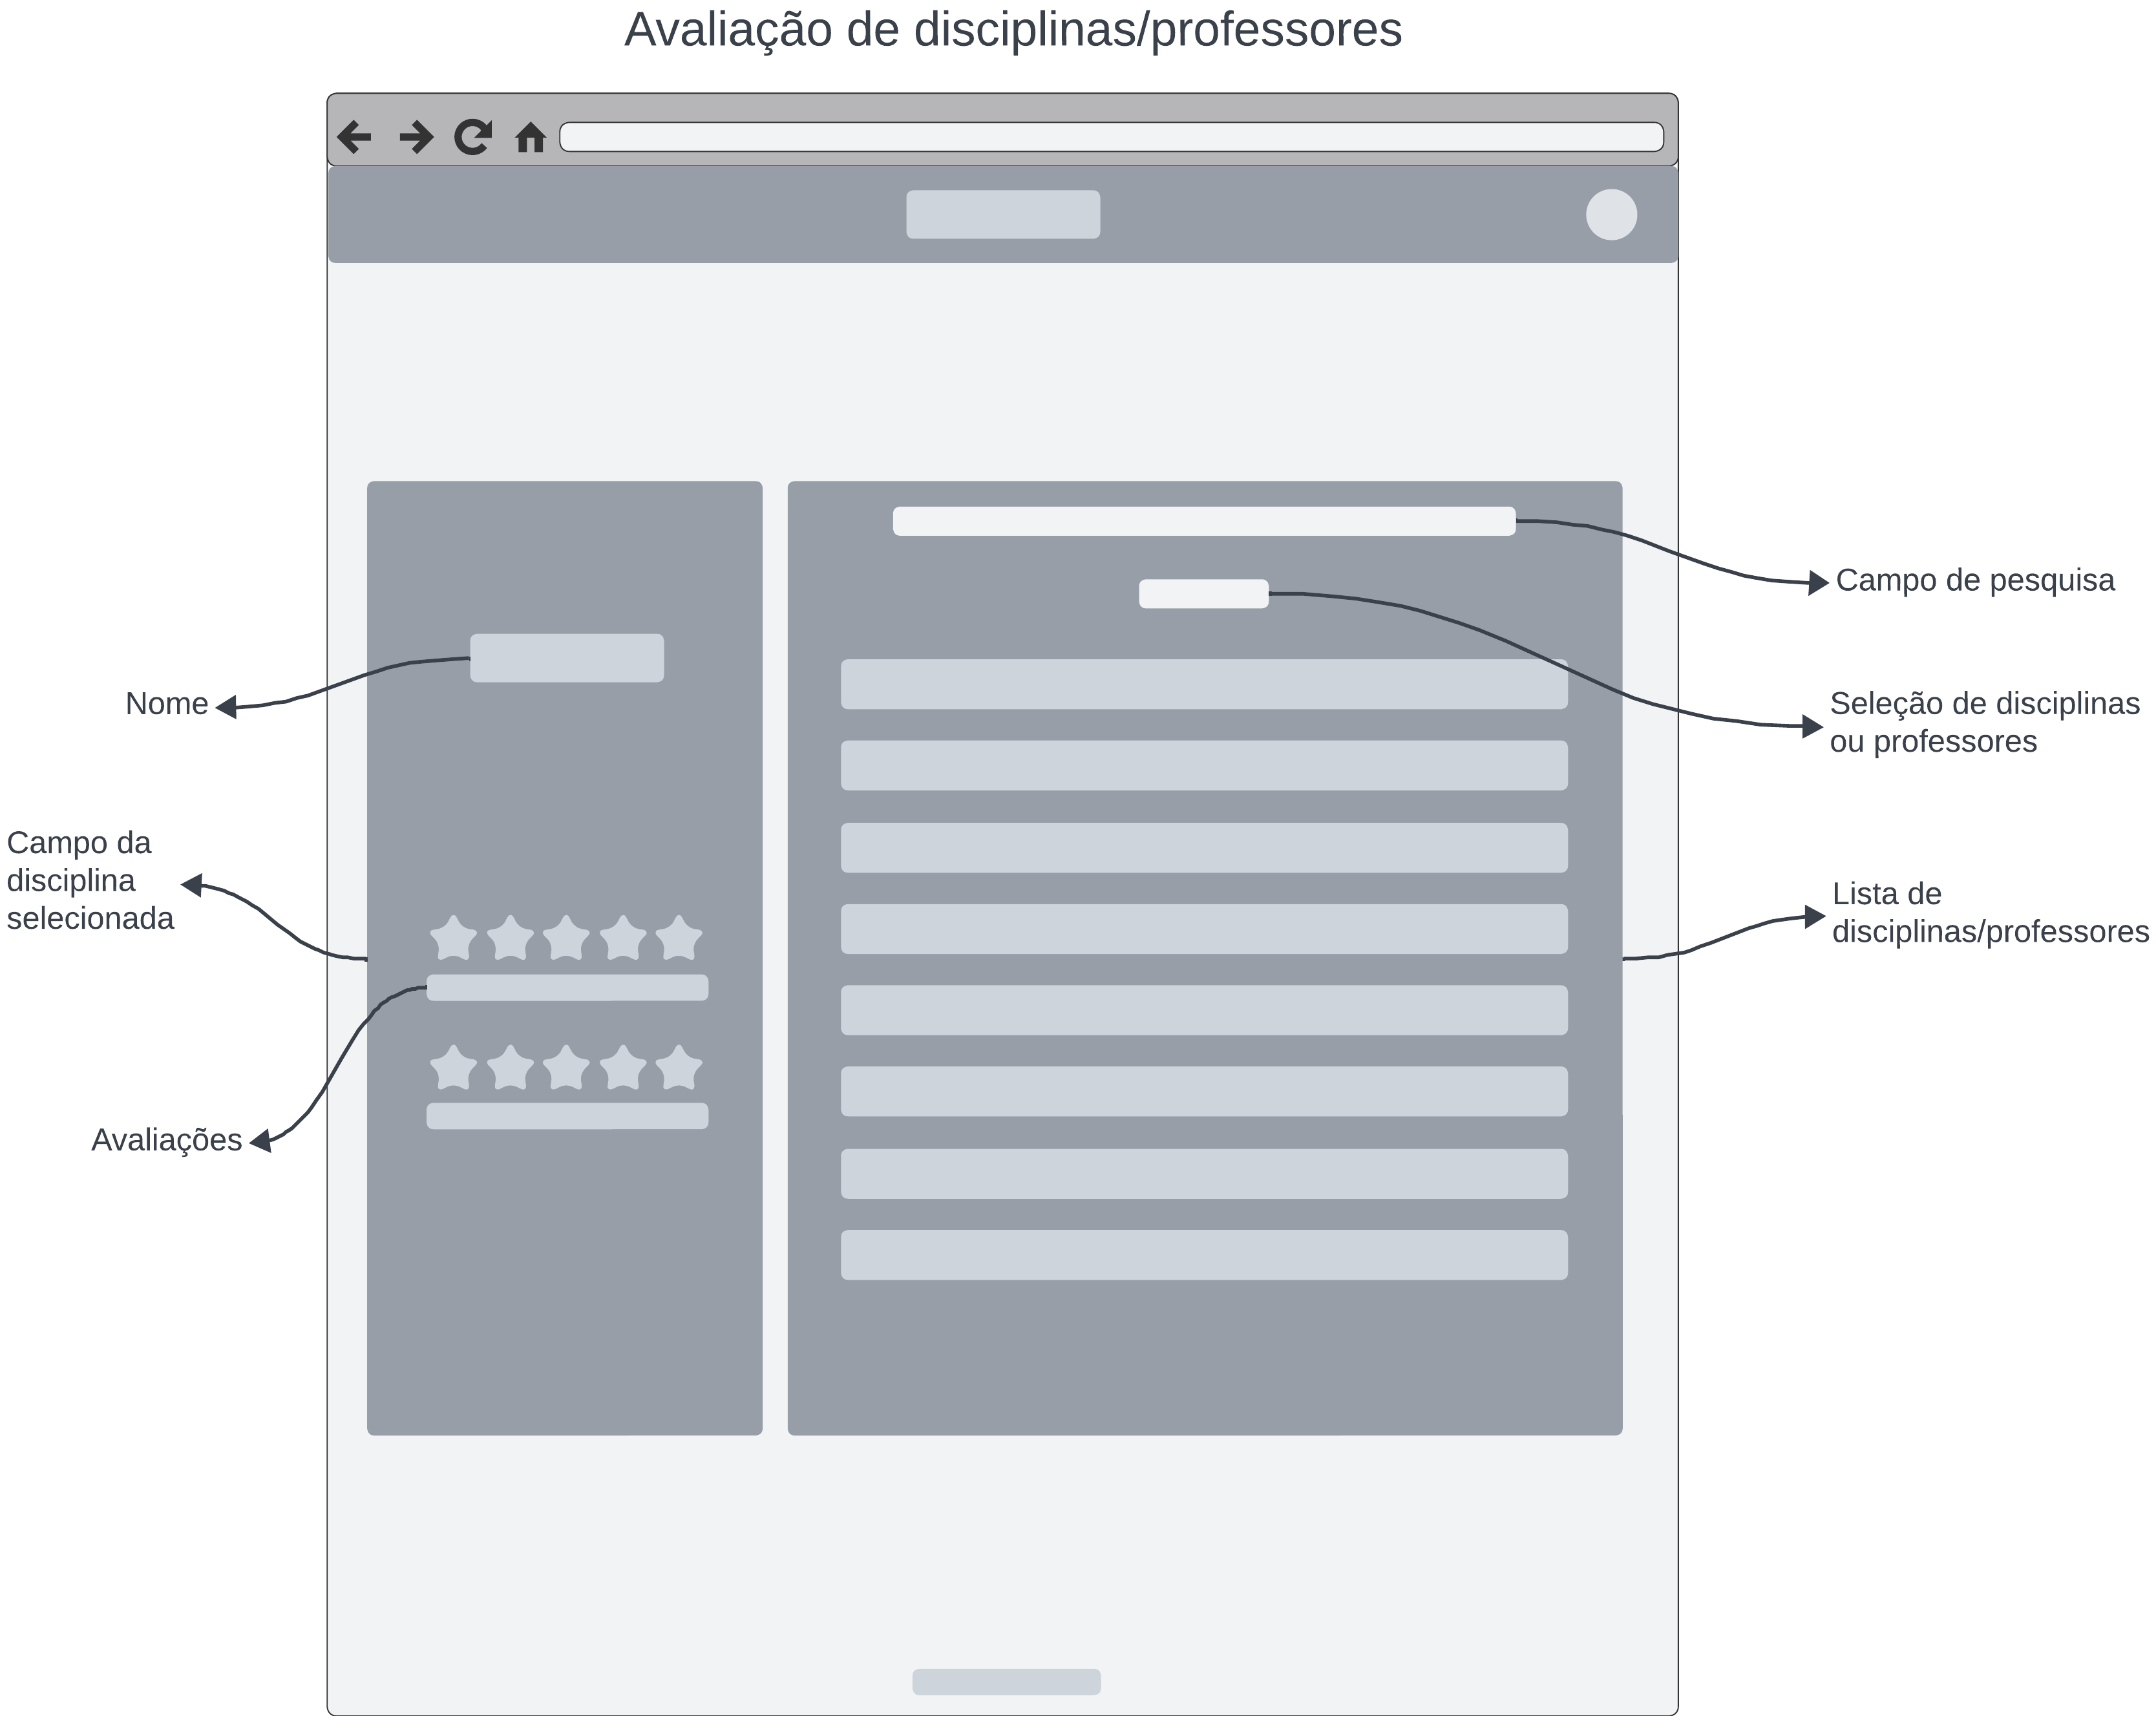
\includegraphics[width=390pt]{figuras/pagina-avaliacao.png}
    \caption{Wireframe da página de avaliação de disciplinas e professores}
    \label{fig:wireframe-pagina-avaliacao}
    \end{center}
\end{figure}